\documentclass[a4paper,11pt]{article}
\usepackage[utf8]{inputenc}
\usepackage[T1]{fontenc}
\usepackage[frenchb]{babel}

\usepackage{graphicx}
\usepackage{fancyhdr}
\usepackage{geometry}

\usepackage[colorlinks,linkcolor=blue]{hyperref}
\usepackage{amsmath}
\usepackage{amssymb}
\usepackage{mathrsfs}
\usepackage{epsfig}
\usepackage {eurosym}

\usepackage{float}

\geometry{a4paper,tmargin=2cm,bmargin=2cm,lmargin=1.5cm,rmargin=1cm,headheight=2.2cm,headsep=0.5cm,footskip=1cm}
\columnsep=0.6cm

\graphicspath{{images/}} 

\usepackage{listings}
\usepackage{color}
\usepackage{xcolor}

\lstset{columns=flexible,keepspaces=true, breaklines,breakindent=0pt} 


\lstset{language=VHDL,
basicstyle=\ttfamily\footnotesize,
breaklines, 
keywordstyle=\bfseries\color{blue},
stringstyle=\color{red},
commentstyle=\color{blue!20!black!30!green},
morecomment=[s][\color{black}]{/**}{*/},
numbers=left,
numberstyle=\tiny\color{black},
stepnumber=2,
numbersep=10pt,
tabsize=4,
showspaces=false,
showstringspaces=false}


\fancypagestyle{plain}{
% noms des respo   dans le bas de page                                            
\lfoot{Projet de VHDL}
\rfoot{M.Morin J.Fourmann}
\renewcommand{\headrulewidth}{0pt}
\fancyhead{}}
% Titre a compl»ter
\title{\textbf{ \huge{Projet de VHDL}}  \\{\Large Réalisation d'un Fréquencemètre}}

\author{
\textsc{Jérémie Fourmann} (Promo 2013 - Eléctronique)\\ %mettre votre nom
\textsc{Maxime Morin} (Promo 2013 - Eléctronique)\\ %mettre votre nom
%\textsc{ddd dddd} (Promo - departement - respo)     %2 nom
}

\graphicspath{{images/}}

\begin{document}

\pagestyle{plain}

\maketitle
\begin{center}

\includegraphics[width=6cm]{inp-enseeiht.pdf}   
\end{center}

\vspace{1cm}
\renewcommand{\contentsname}{Plan}
\tableofcontents
\vspace{2cm}

\newpage
\section{Objectifs}
Le but de ce projet est de meusurer la fréquence d'un signal, le résultat de cette mesure sera affichée sur quatres afficheurs 7 segments.\\
\subsection{Rappel du cahier des charges}
Notre projet doit répondre aux contraintes suivantes :
\begin{description}
 \item[Changement de gamme automatique :] Pour garder le plus de précision possible, 
il faudra changer de méthode de mesure quand la fréquence dépassera une certaine valeur (voir partie nos choix).
\item[Rafraichissement de la mesure de 1s :] Permet de garder une bonne fluidité lorsque la fréquence est ammenée à changer.
\item[Affichage sur 4 digits :] Permet d'avoir une précision correcte
\item[Plage de fréquence de 1Hz à 10 MHz]
\item[Affichage des calibres]  
\end{description}
\vspace{.5cm}
\emph{RQ: Par ailleurs notre système affichera un message d'alerte quand le signal mesuré dépasse la plage de fréquence admise.}

\subsection{Nos choix}
\subsubsection{Choix de la validité des méthodes de mesures}
Nous avons deux méthodes de mesures à notre disposition : méthode étalon et méthode échantillonage.\\
\begin{figure}[H]
\begin{center}
	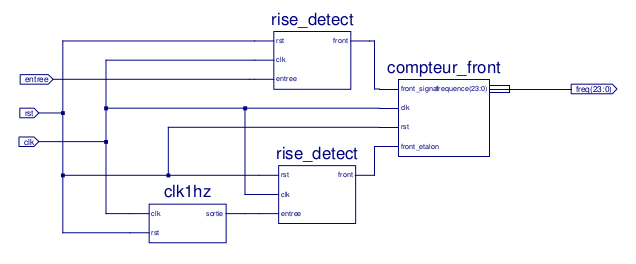
\includegraphics[scale=.3]{etalon.png}
	\caption{Métode étalon}
\end{center}
\end{figure}

\begin{figure}[H]
\begin{center}
	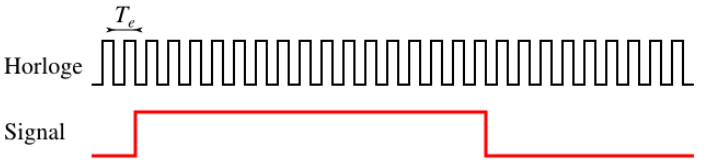
\includegraphics[scale=.3]{ech.png}
	\caption{Méthode échantillonage}
\end{center}
\end{figure}
Ces deux méthodes ne sont pas meilleur l'une que l'autre, elles sont complémentaires.\\
En effet pour un signal de fréquence élevé nous utiliseron la méthode étalon, elle permet d'avoir le maximum de précision.\\
En revanche à basse fréquence cette méthode ne peut s'apliquer convenablement, nous utilisons alors la méthode échantillonage.\\

Il faut donc trouver la valeur pour laquelle on change de méthode de mesure. Nous allons tracer la précision en fonction de la fréquence pour 
les deux méthodes\\
On a :
\begin{equation*}
 Precision_{BF}=\frac{F_{clk}}{F_{signal}}
\end{equation*}
\begin{equation*}
 Precision_{HF}=\frac{F_{signal}}{F_{étalon}}
\end{equation*}

\begin{figure}[H]
\begin{center}
	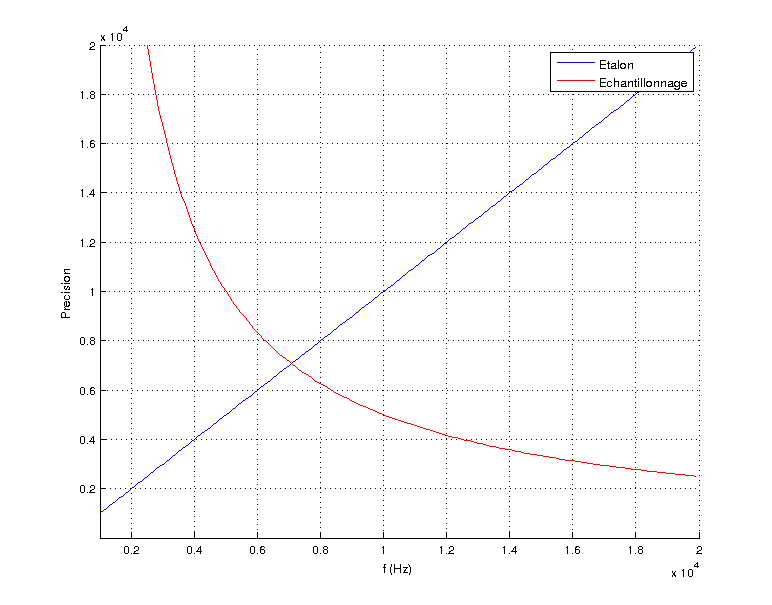
\includegraphics[scale=.5]{graphMethode.png}
	\caption{Précision des deux méthodes}
\end{center}
\end{figure}
On s'aperçoit que pour avoir le maximun de précision il faut changer de méthode aux alentours de 7 KHz. 

\subsubsection{Choix de la conception en machine d'état}
Notre conception étant entièrement synchrone, chaque sous module de notre sytème sera une machine d'état avec le bloc M et G synchronisé sur
la clock du FPGA.\\
Cette conception en machine d'état nous assure une implémentation adapté aux fonctionement du FPGA.\\ 
Par ailleurs nous avons aussi une meilleur lisibilité de notre programme et une meilleur facon de débugger car nous avons accès à l'état de notre machine lors des simulations.\\
\newpage
\section{Conception du système}

\subsection{Présentation du système}
\subsection{Présentation des sous Modules}
\subsubsection{Schéma bloc}
\subsubsection{Machine d'état}
\subsubsection{Résulat de simulation}

\subsection{Performance du système}

\newpage
\section{Bilan}

\newpage
\appendix
\section{Manuel d'utilisateur}
\subsection{Introduction}
L'utilisateur pourra utilisé le projet soit en utilisant le component Fréquencemètre pour l'inclure dans un autre projet soit l'utilisé directement sur la Nexys 2.

\subsection{Component VHDL}
Notre projet peut se résumer en un seul component suivant :


\subsection{Implémentation sur Nexys 2}
En chargent le .bit, l'utilisateur pourra utilisé le fréquencemètre.
\begin{figure}[H]
\begin{center}
	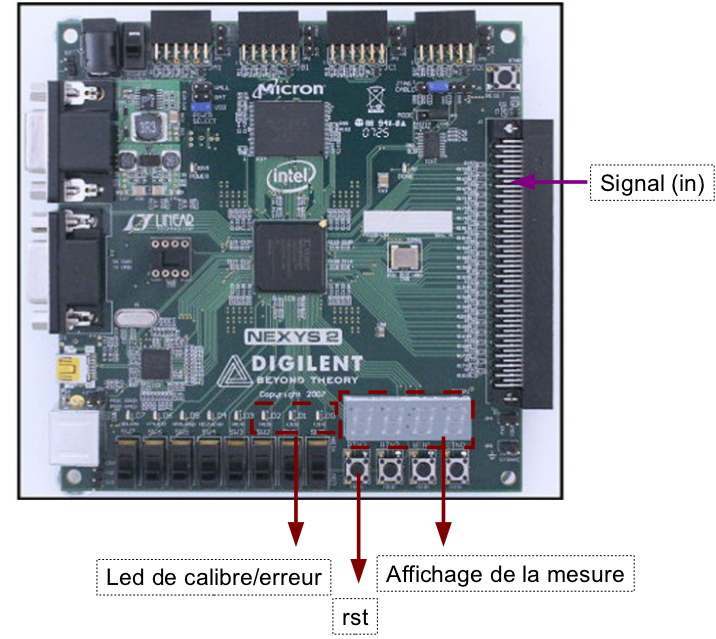
\includegraphics[scale=.5]{fpga.png}
	\caption{Implémentation sur carte Nexys 2}
\end{center}
\end{figure}

\subsection{Fichier contrainte}
L'utilisateur pourra édité le fichier de contraintes selon ses besoins et ressources disponible.
\lstinputlisting{../frequencemetre.ucf}
\newpage
\section{Extrait de code VHDL}
\lstinputlisting{../machine_etat.vhd}
\end{document}
